\section{Second Trajectory}
The second trajectory to complete the task seen in \autoref{fig:secondTask} is different that the first, in that it does not require movement in the ($\theta$, $\dot{\theta}$)-plane, in fact, rather the contrary. It does however require the cart to move forward in order to pass the obstacles and hold up the pendulum.\\
As before, the initial values are known and a final position of the cart can be chosen, which will be the condition for switching to the final task.\\
Substituting the initial values, $\theta = \theta_t$ (target angle), $\dot{\theta} = 0$ and $\ddot{\theta} = 0$, into the dynamic equations, \autoref{eq:dynamicEquation1} and \autoref{eq:dynamicEquation1}, reduces to,
%
\begin{flalign}
  m l \cos \theta_t \ \ddot{x} - m l g \sin \theta_t &=  0  & %\unit{N \cdot m}  \\
  \label{eq:dynamicEquation1SecondTrajectory} \\
  (M+m) \ddot{x} &=  f  \ \ \ . & %\unit{N \cdot m}
  \label{eq:dynamicEquation2SecondTrajectory}
\end{flalign}

In \autoref{eq:dynamicEquation2SecondTrajectory} the force, $f$, is directly provided as a function of the acceleration of the cart. Feeding back $\ddot{x}$ in this manner will attempt to keep the angle of the pendulum steady while moving forward through the obstacles.\\
It is interesting to note that the average of the force excreted during this second trajectory changes the $\theta$-dynamics in such a way that the angle and angular velocity are kept in a saddle point equilibrium.

\begin{figure}[H]
  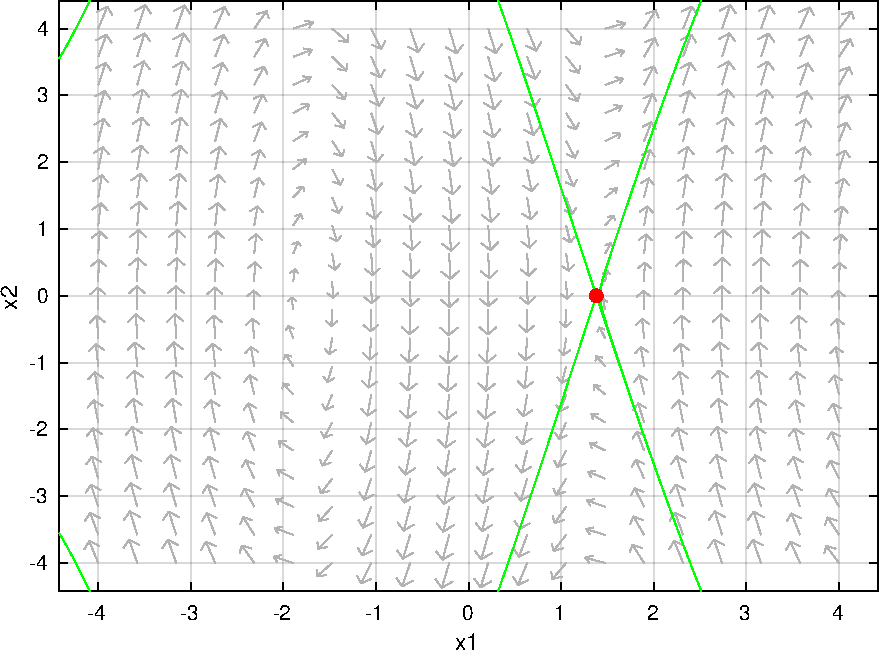
\includegraphics[width=.6\textwidth]{figures/secondTrajectory}
  \caption{Phase portrait showing how the $\theta$-dynamics changes given a constant force averaged from the forces used during the second trajectory. The system is kept near the indicated saddle point equilibrium.}
  \label{fig:phasePortraitSecondTrajectory}
\end{figure}